\chapter{Исследовательская часть}

\section{Технические характеристики}
Характеристики используемого оборудования:
\begin{itemize}
    \item операционная система --- Windows 11 Home
    \item память --- 16 Гб.
    \item процессор --- 12th Gen Intel(R) Core(TM) i7---12700H @  2.30 ГГц~\cite{intel}
\end{itemize}

\section{Время выполнения алгоритмов}

Замеры времени проводились на графах с одинаковым количеством вершин. Каждое значение получено путем взятия среднего из 10 измерений. Зависимости времени решения задачи коммивояжера от количества вершин графа для двух алгоритмов представлены на рисунке~\ref{fig:time_mes}.

\begin{figure}[H]
    \centering
    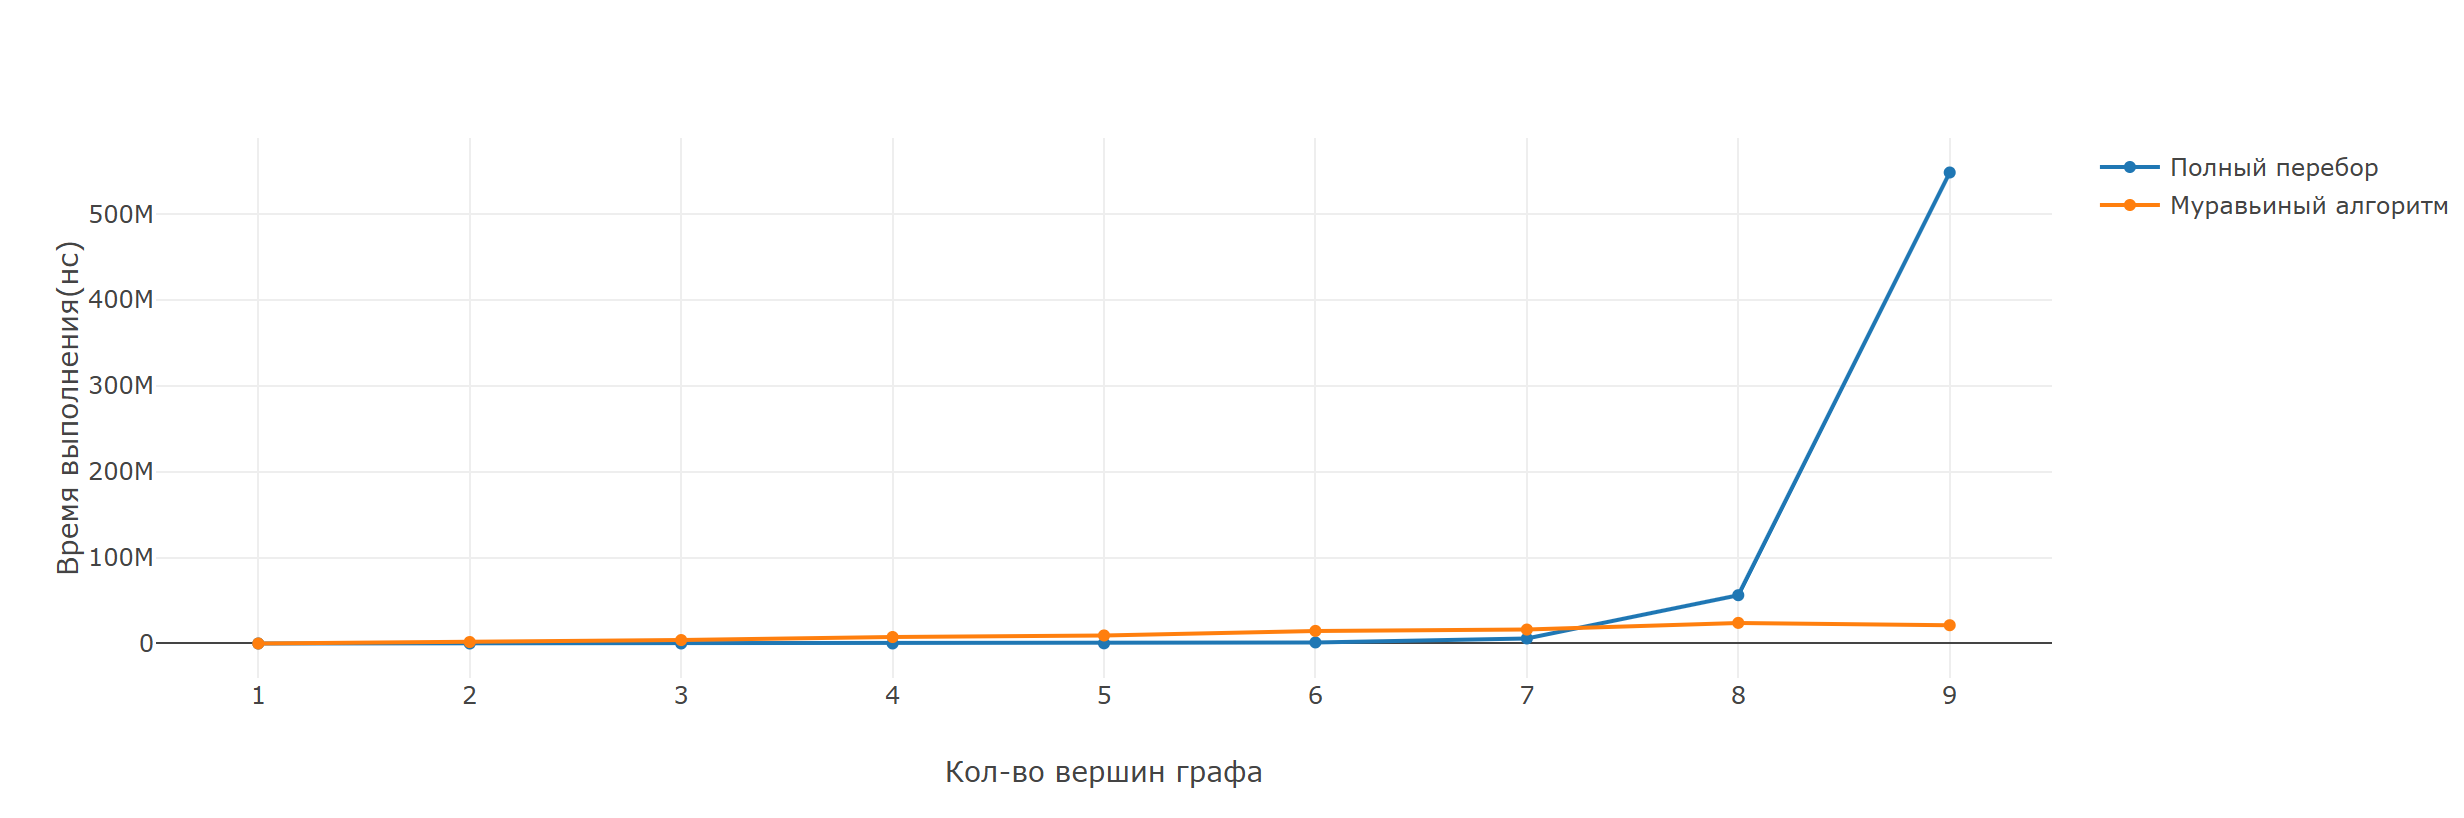
\includegraphics[width=1\linewidth]{images/plot.png}
    \caption{Сравнение алгоритмов по времени}
    \label{fig:time_mes}
\end{figure}

\section{Результаты параметризации}

В результате параметризации оказалось, что самыми лучшими параметрами по заданному классу данных оказались при $\alpha$ = 0.75, $\rho$ = 0.1 и количеством дней равным 200. При этом данные параметры дают лучший результат на всех классах данных и по всем параметрам сравнения. Результаты параметризации для лучших параметров представлены в таблице~\ref{tbl:param}, а
вся таблица параметризации и класс данных представлены в приложении А.


\begin{longtable}{|r|r|r|r|r|r|r|r|r|r|r|r|}
\caption{Результаты параметризации муравьиного алгоритма}\label{tbl:param}
\\ \hline
\multicolumn{3}{|c|}{Параметры} & \multicolumn{3}{|c|}{Граф 1} & \multicolumn{3}{|c|}{Граф 2} & \multicolumn{3}{|c|}{Граф 3} \\
\hline
$\alpha$ & $\rho$ & Дни & min & max & avg & min & max & avg & min & max & avg \\
\hline
\endfirsthead
\hline
\endhead
\hline
\endfoot
\endlastfoot
\hline
0.50 & 0.50 & 200 & 0.00 & 0.00 & 0.00 & 0.00 & 0.00 & 0.00 & 0.00 & 0.00 & 0.00  \\
\hline
0.75 & 0.10 & 100 & 0.00 & 0.00 & 0.00 & 0.00 & 0.00 & 0.00 & 0.00 & 0.00 & 0.00  \\
0.75 & 0.10 & 200 & 0.00 & 0.00 & 0.00 & 0.00 & 0.00 & 0.00 & 0.00 & 0.00 & 0.00  \\
\hline
\end{longtable}


\paragraph*{ВЫВОД} ${}$ \\

Результаты измерений времени показали, что на графа с вершинами меньше 8 муравьиный алгоритм уступает алгоритму полного перебора менее чем в 2.2 раза. Однако с увеличением количества вершин графа муравьиный алгоритм демонстрирует значительное преимущество. На графах с количеством вершин больше 7 муравьиный алгоритм работает быстрее более чем в 2.5 раз. Для проведения замеров времени количество дней в муравьином алгоритме было установлено равным 200.

Также в данном разделе была проведена параметризация и выявлены лучшие параметры для заданного в приложение А классов данных.